\documentclass[12pt, a4paper, oneside]{ctexbook}
\usepackage{amsmath, amsthm, amssymb, bm, graphicx, hyperref, mathrsfs}

\title{{\Huge{\textbf{机器人运动控制重点整理}}}}
\author{陈傲}
\date{\today}
\linespread{1.5}
\hypersetup{
	colorlinks=true,
	linkcolor=black
}
\begin{document}

\maketitle

\pagenumbering{roman}
\setcounter{page}{1}

\begin{center}
    \Huge\textbf{前言}
\end{center}~\

这本书作为这门课的重点整理,主要是面向考试,以及考前的复习。所以,使用这本书需要你有一定的基础,用这本书来进行复习,而不是用它来进行日常的学习。这本书中会缩减大量内容,如简单、学一遍就会内容不会列出,而且这本书中只给出结论,方便考前记忆背诵。

若你想学习这门课,推荐去看我的笔记和b站录制的配套视频:《机器人运动控制简明教程》。这本书与笔记已全部开源。

仓库地址:https://github.com/DylanAo/AHU-AI-Repository。
~\\
\begin{flushright}
    \begin{tabular}{c}
        陈傲\\
        于槐园\\
        \today
    \end{tabular}
\end{flushright}

\newpage
\pagenumbering{Roman}
\setcounter{page}{1}
\tableofcontents
\newpage
\setcounter{page}{1}
\pagenumbering{arabic}
\chapter{重点内容背诵}
\section{公式背诵}
\begin{align}
	&^{A}p=^{B}p+^{A}p_B\\
	&^{B}p=^{B}_{A}R {\quad} ^{A}p\\
	&(^{A}_{B}R)^{T}=(^{A}_{B}R)^{-1}
\end{align}
\begin{align}
	\left[
	\begin{matrix}
		^{A}p\\
		1
	\end{matrix}
	\right]=&
	\left[
	\begin{matrix}
		^{A}_{B}R & ^{A}P_B\\
		0 & 1
	\end{matrix}
	\right]
	\left[
	\begin{matrix}
		^{B}p\\
		1
	\end{matrix}
	\right]\\
	\left[
	\begin{matrix}
		\mbox{变换后的坐标}\\
		1
	\end{matrix}
	\right]=&
	\left[
	\begin{matrix}
		\mbox{旋转变换矩阵} & \mbox{平移矩阵}\\
		0 & 1
	\end{matrix}
	\right]
	\left[
	\begin{matrix}
		\mbox{变换前坐标}\\
		1
	\end{matrix}
	\right]
\end{align}
\begin{align}
	&R(x,\theta)=
	\left[
	\begin{matrix}
		1 & 0 & 0\\
		0 & \cos(\theta) & -\sin(\theta)\\
		0 & \sin(\theta) & \cos(\theta)
	\end{matrix}
	\right]\\
	&R(y,\theta)=
	\left[
	\begin{matrix}
		\cos(\theta) & 0 & \sin(\theta)\\
		0 & 1 & 0\\
		-\sin(\theta) & 0 & \cos(\theta)
	\end{matrix}
	\right]\\
	&R(z,\theta)=
	\left[
	\begin{matrix}
		\cos(\theta) & -\sin(\theta) & 0\\
		\sin(\theta) & \cos(\theta) & 0\\
		0 & 0 & 1
	\end{matrix}
	\right]
\end{align}
\begin{align}
	dT=&\delta T\\
	\delta = Trans(dx,dy,dz)&Rot(r,d\theta)-I_{4\times4}
\end{align}
\begin{align}
	V&=J(\theta)\dot{\theta}\\
	\dot{\theta}&=J^{-1}V\\
	\tau&=J^T F
\end{align}
\begin{align}
	\mbox{拉格朗日函数} &\qquad L=T-V\\
	\mbox{拉格朗日方程} &\quad \tau_i=\frac{d}{dt}\frac{\partial L}{\partial \dot{q_i}}-\frac{\partial L}{\partial q_i}
\end{align}

\section{知识点背诵}
\begin{center}
	\textbf{重点掌握:1、4、6、7、13、11、12、13}
\end{center}

\begin{enumerate}
	\item 机器人由机械本体、驱动部分和传感和控制三个基本部分组成。本体即机座和执行机构,如机械手的臂部、腕部和手部,有的机器人还有行走机构。大多数工业机器人有3-6个运动自由度,其中腕部通常有1-3个运动自由度;驱动系统包括动力装置和传动机构,用以使执行机构产生相应的动作;控制系统可以按照输入的程序对驱动系统和执行机构发出指令信号,并进行操作控制。
	\item 控制系统性能在很大程度上决定了机器人的整体性能。
	\item 机器人控制系统的基本要素包括电动机、减速器、运动特性检测传感器、驱动电路、控制系统硬件和软件。
	\item 机器人位置运动学包括正运动学和逆运动学,正运动学即给定机器人各关节变量,计算机器人末端的位置姿态;逆运动学即已知机器人末端的位置姿态,计算机器人对应位置的全部关节变量。一般正运动学的解是唯一和容易获得的,而逆运动学往往有多个解,而且分析更为复杂。
	\item 机器人分类:
	
	(1)按几何结构分类-利用坐标特性分类:直角坐标机器人:由互相垂直的导轨和手臂构成;柱面坐标机器人:主要由垂直柱子、水平手臂和底座构成。工作区间为圆柱面;球面坐标机器人:由底座、球关节和手臂构成。其工作区间为球面。其中,最常见的是关节式球面坐标机器人,由躯干、上臂和前臂构成。
	
	(2)按几何结构分类-利用机构特性分类:串联机器人:各连杆为串联;并联机器人:各连杆为并联。
	
	(3)按几何结构分类-利用尺寸分类:大型机器人;一般机器人;微机器人。
	
	
	(4)按应用领域分类:工业机器人:应用于工农业生产,主要应用于制造业,如弧焊机器人、喷漆机器人、装配机器人等;服务机器人:一种自主或半自主工作,为人们提供服务的机器人,如导游机器人、家用机器人等;探索机器人:用于太空、海洋、地下探险和探索;军事机器人:用于军事目的。可分为陆、海、空军用机器人。如无人战机、机器人战士等。
	我国按照应用领域将机器人分为:工业机器人、服务机器人、特种机器人。
	
	(5)按智能程度分类:一般机器人:只有一般编程能力和操作功能;智能机器人:根据智能程度分为:传感型、交互型、自主型智能机器人。
	
	(6)按机器人的移动性分类:固定式机器人:固定在底座上,如工业机器人;移动机器人:根据移动方式分为:轮式、履带式、足式等。如足式机器人中的人形机器人等。
	
	\item 机器人控制的特点
	
	(1)非线性:
	机构构型、传动机构、驱动元件等都会引起系统的非线性。
	
	(2)多变量:
	机器人系统是一个时变系统,动力学参数随着关节运动位置的变化而变化。
	
	(3)强耦合:
	各关节具有耦合作用,表现为某一个关节的运动,会对其他关节产生动力效应,使得每个关节都要承受其他关节运动所产生的扰动。
	
	总结:机器人是一个十分复杂的多输入多输出非线性系统,且在实际应用中一般很难得到精确的动力学方程
	
	为解决以上问题,我们将复杂的整体控制问题简化为多个低阶子系统的控制问题;将控制分为单关节控制、多关节控制问题,这样前者需要考虑误差补偿问题,后者考虑耦合作用的补偿。由于工业机器人通常运动速度比较低,也要安装减速器,所以工业机器人系统就变成了一个由多关节(多轴)组成的各自独立的线性系统。
	
	\item 机器人控制方法: 滑模控制、模糊控制、人工神经网络控制、遗传算法、自适应控制、PID控制。
	
	\item 机器人控制的性能要求:稳快准。
	
	稳定性:当系统受到的扰动撤离后,系统仍能回到原有的平衡状态。
	
	响应速度:瞬态响应具有一定的快速性和平稳性。
	
	稳态精度:给定稳态误差:在参考输入信号作用下,系统稳定后,稳态输出与期望输出之差。扰动稳态误差:在扰动信号作用下,系统稳定后,输出量与期望输出之差。
	
	\item PID:
	
	比例(P)调节作用:按比例反映当前系统的偏差。系统一旦出现了偏差,比例调节立即产生调节作用用以减少偏差。减小响应曲线上升时间,加快系统的响应,有利于减小静态误差。
	
	积分(I)调节作用:是过去系统误差的积累。使系统消除稳态误差,提高无差度。因为有误差,积分调节就进行,直至无差,积分调节停止,积分调节输出一常值。减小系统稳态误差,减小振荡,使系统的稳定性增加。
	
	微分(D)调节作用:反映未来系统偏差信号的变化率,具有预见性,能产生超前的控制作用。可以减少超调,减少调节时间,改善系统的动态性能。微分作用对噪声干扰有放大作用,因此过强的加微分调节,对系统抗干扰不利。影响系统的响应速度,使系统超调量减小,增强系统稳定性。
	
	\item 被动柔顺:机器人凭借一些辅助的柔顺机构(如弹簧),使其在与环境接触时能够对外部作用力产生自然顺从。
	
	\item 主动柔顺:机器人利用力的反馈信息采用一定的控制策略去主动控制作用力。
	
	\item 柔顺控制:柔顺控制就是从(力)传感器取得控制信号,用此信号控制机器人,使之响应外界的变化而动作。
	
	\item 柔顺控制策略
	
	(1)\textbf{力/位混合控制}:
	
	将任务空间划分成两个正交互补的子空间——力控制子空间和位置控制子空间,在力控制子空间中用力控制策略进行力控制,在位置控制子空间中利用位置控制策略进行位置控制。核心思想是分别用不同的控制策略对位置和力直接进行控制,即首先通过选择矩阵确定当前接触点的位控和力控方向,然后应用力反馈信息和位置反馈信息分别在位置环和力环中进行闭环控制,最终在受限空间中实现力和位置的同时控制。
	
	
	(2)\textbf{阻抗/导纳控制}:
	
	a.阻抗:将外界接触环境等效为导纳,其输入为接触力,输出为运动响应;而将机器人等效为阻抗,其输入为运动响应,输出为接触力。这样机器人与环境系统的行为类似于一个匹配的阻抗电路,机器人力控制问题便成了阻抗调节问题,即通过位置的调整来实现力的控制。
	
	b.导纳:控制系统采用基于位置控制的内环和力控控制的外环策略。检测系统与外界的接触力,通过一个二阶导纳模型,生成一个附加的位置,再用此附加位置去修正预先设定的位置轨迹,最终送入位置控制内环,完成最终的位置控制。
	
	(3)\textbf{模型参考自适应控制}:
	
	将机器人实际的行为(实际模型)与参考模型进行比较,计算出系统误差。这个系统误差代表了机器人当前行为与期望行为之间的差异。根据系统误差,控制器会自适应地调整其控制参数,以减小误差。控制参数会不断地进行自适应调整,以达到柔顺控制目的。
	
	
\end{enumerate}

\chapter{重点内容详解}

\section{坐标变换:平移与旋转}

\subsection{平移与旋转变换规律}
平移:对于平移而言,点p在A坐标系下位置等于点p在B坐标系下位置加上A,B坐标系间相对值(也就是你要平移的量),角标也相当于可约。
换句话硕,平移就等于原来的矩阵加上平移后的矩阵。
$$
^{A}p=^{B}p+^{A}p_B
$$

旋转:旋转要遵守\textbf{右乘连体左乘基}的规则,要注意其角标是可以\textbf{约掉的}。
$$
^{B}p=^{B}_{A}R {\quad} ^{A}p
$$

旋转变换矩阵不仅可以描述旋转,其本质上也可描述刚体在坐标系中姿态。同时还有逆等于转置的性质:
$$
(^{A}_{B}R)^{T}=(^{A}_{B}R)^{-1}
$$

请注意:\textbf{这种可以约掉性质是最重要的性质},在做题时要根据可以约掉性质判断出不同坐标系间不同关系。
\subsection{绕XYZ轴的旋转变换矩阵}

$$
R(x,\theta)=
\left[
\begin{matrix}
	1 & 0 & 0\\
	0 & \cos(\theta) & -\sin(\theta)\\
	0 & \sin(\theta) & \cos(\theta)
\end{matrix}
\right]
$$

$$
R(y,\theta)=
\left[
\begin{matrix}
	\cos(\theta) & 0 & \sin(\theta)\\
	0 & 1 & 0\\
	-\sin(\theta) & 0 & \cos(\theta)
\end{matrix}
\right]
$$

$$
R(z,\theta)=
\left[
\begin{matrix}
	\cos(\theta) & -\sin(\theta) & 0\\
	\sin(\theta) & \cos(\theta) & 0\\
	0 & 0 & 1
\end{matrix}
\right]
$$
\subsection{齐次坐标变换}

$$
\left[
\begin{matrix}
	^{A}p\\
	1
\end{matrix}
\right]=
\left[
\begin{matrix}
	^{A}_{B}R & ^{A}P_B\\
	0 & 1
\end{matrix}
\right]
\left[
\begin{matrix}
	^{B}p\\
	1
\end{matrix}
\right]
$$

$$
\left[
\begin{matrix}
	\mbox{变换后的坐标}\\
	1
\end{matrix}
\right]=
\left[
\begin{matrix}
	\mbox{旋转变换矩阵} & \mbox{平移矩阵}\\
	0 & 1
\end{matrix}
\right]
\left[
\begin{matrix}
	\mbox{变换前坐标}\\
	1
\end{matrix}
\right]
$$
$$
^{A}p^{'}=^{A}_{B}T {\quad} ^{B}p^{'}
$$

同时,我们的齐次坐标变换矩阵还有以下性质:
$$
(^{A}_{B}T)^{-1}=^{B}_{A}T
$$

注意:

1. 齐次坐标变换矩阵是一个$4\times4$矩阵。

2. 因为矩阵乘法没有交换律存在,所以导致先旋转后平移其齐次坐标变换矩阵为$\left[
\begin{matrix}
	^{A}_{B}R & ^{A}P_B\\
	0 & 1
\end{matrix}
\right]$,而先平移后旋转则变成$\left[
\begin{matrix}
	^{A}_{B}R & ^{A}_{B}R^{A}P_B\\
	0 & 1
\end{matrix}
\right]$,所以我们一定要分开来计算。
\section{DH参数法}
\subsection{DH参数及其物理意义}
关节轴线:第$i$个关节的轴线记为$J_i$。

连杆长度:两个关节的关节轴线$J_i$与$J_{i+1}$的公垂线距离为连杆长度,记为$a_i$。

连杆扭转角:由$J_i$与公垂线组成平面P,$J_{i+1}$ 与平面P的夹角为连杆扭转角,记为$ \alpha_i$。这里的公垂线指的是$J_i$与$J_{i+1}$间的公垂线。

连杆偏移量:除第一和最后连杆外,中间的连杆的两个关节轴线$J_i$与$J_{i+1}$间都有一条公垂线,一个关节的相邻两条公垂线$a_i$与$a_{i-1}$的距离为连杆偏移量,记为$d_i$。

关节角:关节$J_i的$相邻两条公垂线$a_i$与$a_{i-1}$在以$J_i$为法线的平面上的投影的夹角为关节角,记为$\theta_i$。
\begin{figure}[htbp]
	\centering
	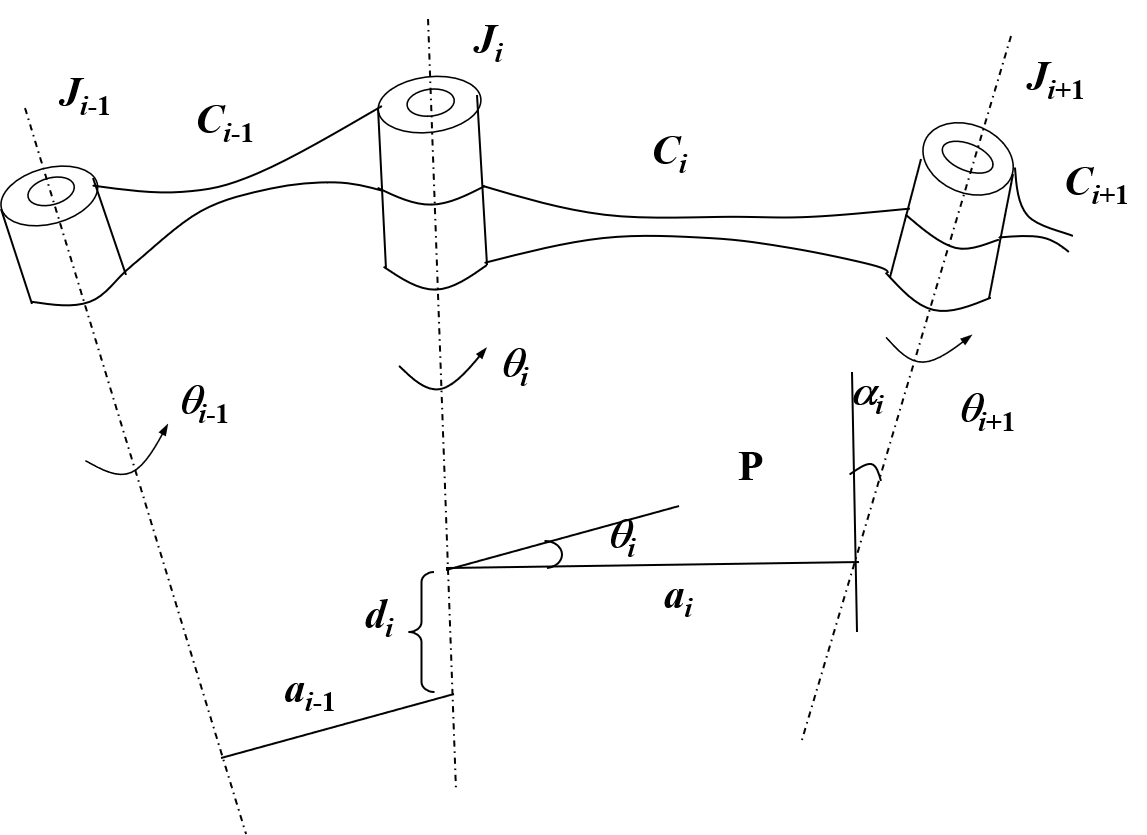
\includegraphics[width=8cm,height=6cm]{img/1.png}
\end{figure}
\newpage
\subsection{连杆坐标系建立简述}
在连杆坐标系中,原点选取就是两种情况:

1.$J_{i+1}$处是原点$O_i$。(标准)

2.$J_{i}$处是原点$O_i$

你建立的坐标系$xyz$轴下标都要与$O_i$下标$i$对应,而不是与关节轴线$J$下标对应。

Z轴就取关节轴线$J$的方向,X轴取公垂线方向,指向下一个连杆,Y轴用右手定则取,使三个轴互相垂直。

\subsection{连杆变换矩阵}

所谓连杆变换矩阵,就是建立连杆坐标系,每个相邻间坐标系进行变换所称的矩阵就是连杆变换矩阵。多个连杆变换矩阵在一起是连体坐标系,需右乘。

要想将$C_{i-1}$坐标系变为$C_i$坐标系,需要经历如下几个变换步骤:

1. 以$Z_{i-1}$轴为转轴,旋转$\theta_i$角度,使旋转后的的$X_{i-1}$轴与$X_i$轴同向。

2. 沿$Z_{i-1}$轴平移$d_i$,使移动后的$O_{i-1}$移动到关节轴线$J_i$与$J_{i+1}$的公垂线在与$J_i$的交点。其实就是往上移动了一下,移动到$O_i$一个高度去了。

3. 沿新的(旋转后)的$X_{i-1}$轴平移$a_i$,使新的$O_{i-1}$移动到$O_i$ 。

4. 以$X_i$轴为转轴,旋转$\alpha_i$角度,使新的$Z_{i-1}$轴与$Z_i$轴同向。
\begin{figure}[htbp]
	\centering
	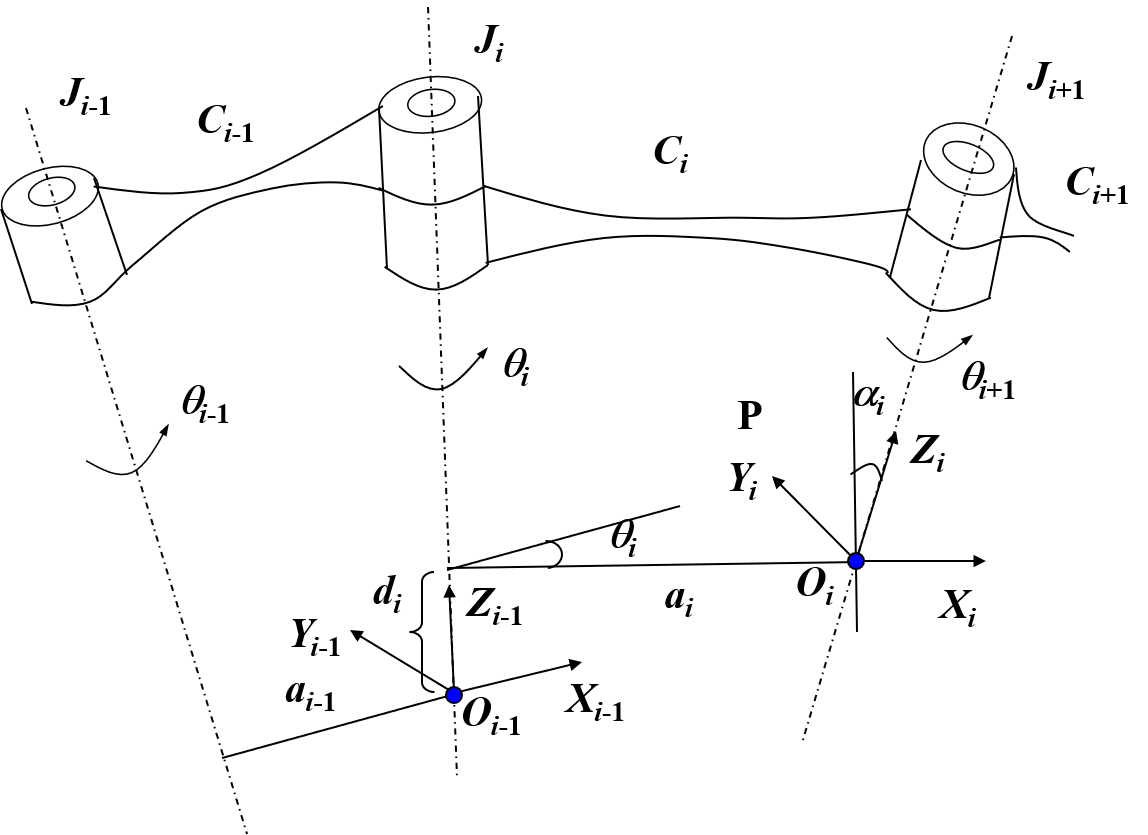
\includegraphics[width=6cm,height=5cm]{img/1_1.png}
\end{figure}
\newpage

\section{微分运动学}
\subsection{微分运动}
机器人某一杆件相对于基座坐标系的位姿为$T$,经过微分运动后该杆件相对基座坐标系的位姿变为$T+dT$,那么有:
$$
dT=\Delta·T
$$
$$
\Delta=Trans(d_X,d_y,d_z)Rot(r,d\theta)-I_{4\times4}
$$

$Rot(r,d\theta)$就是把$sin$直接换成$d\theta$,$cos$直接换成1。
\subsection{雅可比矩阵}
速度雅可比矩阵:
$$
V=J(\theta)\dot{\theta}
$$
$$
\dot{\theta}=J^{-1}V
$$

力雅可比矩阵:
$$
\tau = J^T F
$$
$\tau$为广义关节力矩阵,$F$为首部端点力,$J^T$称力雅可比矩阵。

雅可比矩阵的行数等于机器人操作空间的维度,列数等于机器人的关节数,而且不一定是方阵。对于n关节的机器人来说,雅可比矩阵是$6\times n$的矩阵,前三行代表末端线速度的映射,后三行代表末端角速度的映射。

\section{拉格朗日法}
$$
\mbox{拉格朗日函数} \qquad L=T-V
$$
$T$为系统的总动能,$V$为系统的总势能。
那么我要是像求力或者力矩,就用以下方程,也叫动力学方程:
$$
\mbox{拉格朗日方程} \quad \tau_i=\frac{d}{dt}\frac{\partial L}{\partial \dot{q_i}}-\frac{\partial L}{\partial q_i}
$$

那么什么时候求的是力,什么时候求的是力矩呢?
当$q_i$是一个转动的变量时候,求的是力矩;当$q_i$是一个移动的变量时候,求的是力。

\chapter{重点内容背诵清单}
\begin{enumerate}
	\item 坐标变换:平移、绕xyz轴的旋转。
	\item 机器人由什么组成?
	\item 机器人的分类。
	\item 机器人控制系统的基础要素。
	\item 齐次坐标变换矩阵各参数的意义,能够写出复合齐次变换矩阵(注意区分先平移后转,还是先转后平移)。
	\item 如何描述刚体在坐标系中姿态?
	\item DH参数法的四个参数及其物理意义,齐次变换矩阵的具体应用(理解手爪坐标系、工件坐标系、机座坐标系)。
	\begin{figure}[htbp]
		\centering
		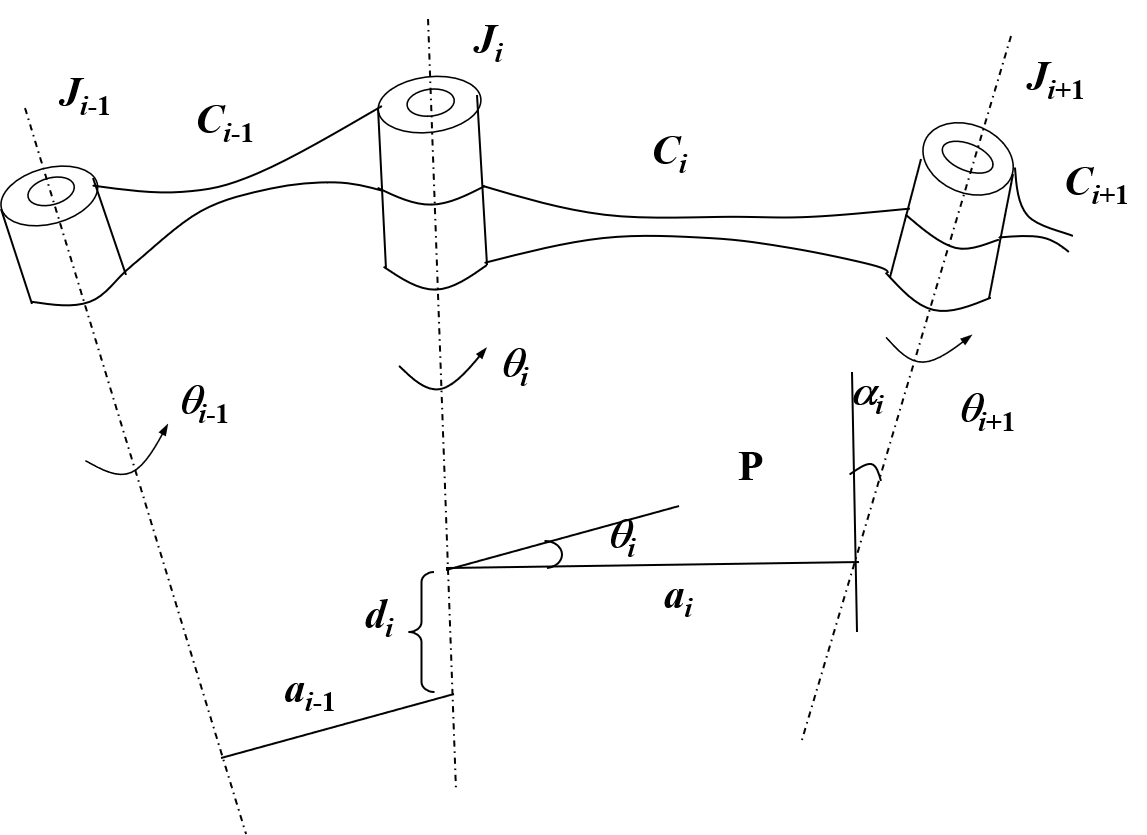
\includegraphics[width=8cm,height=6cm]{img/1.png}
	\end{figure}
	\item 简述正逆运动学的区别,为什么逆运动学问题一般求解复杂,
	\item 微分变化:已知微分转动和平移向量,会写$\delta$,以及与T、T之间的关系。
	\item 雅可比矩阵在机器人运动学和动力学中的应用主要体现在哪几个方面(不少于三点),会计算2自由度机械手的速度雅可比和力雅可比,雅可比矩阵与奇异位形的关系。
	\item 用拉格朗日方法求2自由度机械手的动力学方程。
	\item 结合实例简述机器人控制的特点,列举机器人控制的方法。
	\item 机器人控制的性能要求。
	\item PID有哪些参数,并简述个个参数作用。
	\item 简述主动柔顺和被动柔顺的区别;结合实例论述柔顺控制的目的;列举柔顺控的策略,并简要说明原理。
\end{enumerate}
\end{document}
